\documentclass[12pt]{article}
\usepackage[usenames]{color} %used for font color
\usepackage{amsmath, amssymb, amsthm}
\usepackage{wasysym}
\usepackage[utf8]{inputenc} %useful to type directly diacritic characters
\usepackage{graphicx}
\usepackage [english]{babel}
\usepackage [autostyle, english = american]{csquotes}
\MakeOuterQuote{"}
\graphicspath{ {./} }
\newcommand{\Z}{\mathbb{Z}}
\newcommand{\N}{\mathbb{N}}
\newcommand{\R}{\mathbb{R}}
\newcommand{\Q}{\mathbb{Q}}
\newcommand{\prob}{\mathbb{P}}
\newcommand{\degrees}{^{\circ}}


\author{Tianshuang (Ethan) Qiu}
\begin{document}
\title{Math 74, Week 5}
\maketitle


\section{Mon Lec, 2a}
Let the statement: "There is at most one parallel line to a given line $l$ through a given point $P$." be statement A;
\newline
"If a line intersects one of two parallel lines, both of which are coplanar with the original line, then it also intersects the other." be statement B.
\newline
\begin{figure}[h]
    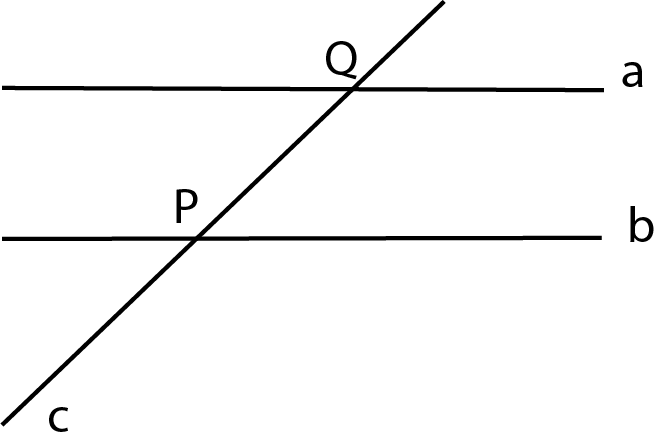
\includegraphics[width = 100mm]{GRAPH1.png}
\end{figure}
We first prove that $A \implies B$. Let $a \parallel b$, and $c$ intersects $a$ at point $Q$. Assume that statement $B$ is false so $c$ does not intersect $b$. Since it does not intersect and $b$ and $c$ are coplanar, we have $b \parallel c$. $a \parallel b$, and $a, c$ interesect at $Q$. However by $A$ we know that there can be at most one line parallel to $b$ at point $Q$. \lightning. Our assumption is incorrect, $A \implies B$

\newline
Then we show that $B \implies A$. Let $a \parallel b$, and $c$ intersects $b$ at point $P$. Assume that $A$ is incorrect, so we construct $a'$ to also be parallel to $b$. We know that $b$ must intersect $a$ by $B$. We name this point $P$. Then since we have assumed that $a \parallel a'$, our line must also intersect $a'$ at $P$.

\section{Mon Lec, 3a}


\section{Mon Dis, 1b}

\subsection{}


\subsection{}

$$\prod^n_i=2 (1-\frac{1}{n^2})$$
We examine $1-1/k^2$ and factor it into $\frac{k^2-1}{k^2} = \frac{(k+1)(k-1)}{k^2}$. Since k is incrementing by 1 in our series, we can cancle each term out. We can expand our series into
$$\frac{1\times 3}{2^2} \frac{2 \times 4}{3^3} ... \frac{(n-1)(n+1)}{n^2}$$
$$= \frac{1}{2} \frac{n+1}{n} = \frac{n+1}{2n}$$

\end{document}
